% ==============================================
% ELEMENTO: DESENVOLVIMENTO
% Pacotes: amsmath, amssymb, booktabs, graphicx, tikz (arrows.meta, positioning, calc)
% \pend marca valores por preencher (a vermelho)
% ==============================================
\providecommand{\pend}{\textcolor{red}{\textbf{?}}}
\section{Desenvolvimento}
\label{sec:desenvolvimento}

% ---------------------------------------------------------------------------
% Seccao 2.1 - Sistema implementado e parametros
% Pacotes necessarios: amsmath, amssymb, booktabs, graphicx, tikz
% (bibliotecas tikz: arrows.meta, positioning, calc)
% ---------------------------------------------------------------------------
\subsection{Sistema implementado e parâmetros}
\label{sec:sistema}

\paragraph{Modelo de sinal.}
O \emph{downlink} é simulado por subportadora. Em OFDM com prefixo cíclico ideal e sincronismo perfeito, cada subportadora vê um canal plano, pelo que cada realização de canal representa uma subportadora e a igualização é feita no domínio da frequência. A estação base tem $N_t$ antenas e serve $K$ utilizadores, o utilizador $k$ com $n_k$ antenas; o número total de antenas receptoras é $N_r=\sum_k n_k$ e, em todos os cenários, $N_s=N_r=N_t$ \emph{streams} (multiplexagem espacial). Para cada subportadora,
\begin{equation}
  \mathbf{y}=\mathbf{H}\,\mathbf{x}+\mathbf{n},\qquad \mathbf{x}=\mathbf{P}\,\mathbf{u},\qquad \hat{\mathbf{u}}=\mathbf{G}\,\mathbf{y},
  \label{eq:modelo}
\end{equation}
onde $\mathbf{H}\in\mathbb{C}^{N_r\times N_t}$ tem elementos independentes $\mathcal{CN}(0,1)$ (canal de Rayleigh), $\mathbf{u}\in\mathbb{C}^{N_s}$ contém os símbolos QPSK ou 16-QAM (mapeamento de Gray, potência média unitária), $\mathbf{P}$ é a matriz de pré-codificação, $\mathbf{G}$ a matriz de recepção e $\mathbf{n}\sim\mathcal{CN}(\mathbf{0},\mathbf{I})$. A SNR por \emph{stream}, $\gamma$, é definida pela potência total transmitida, $\mathbb{E}\|\mathbf{x}\|^2=N_s\gamma$, com ruído de variância unitária em cada antena receptora. A decisão sobre $\hat{\mathbf{u}}$ é feita por limiares, com desmapeamento de Gray.

\paragraph{Pré-codificação.}
$\mathbf{P}$ e $\mathbf{G}$ são calculados a partir do canal conhecido pelo sistema, $\hat{\mathbf{H}}$ (na Fase~1, $\hat{\mathbf{H}}=\mathbf{H}$). Escreve-se a SVD $\hat{\mathbf{H}}=\hat{\mathbf{U}}\hat{\boldsymbol{\Sigma}}\hat{\mathbf{V}}^{H}$, com valores singulares $\sigma_i$.
\begin{itemize}
  \item \textbf{ZF:} $\mathbf{W}=\hat{\mathbf{H}}^{H}(\hat{\mathbf{H}}\hat{\mathbf{H}}^{H})^{-1}$, $\mathbf{P}=\beta\mathbf{W}$ com $\beta^2=N_s\gamma/\|\mathbf{W}\|_F^2$, e $\mathbf{G}=\beta^{-1}\mathbf{I}$. Todos os \emph{streams} ficam com a mesma SNR, $\beta^2$.
  \item \textbf{SVD:} $\mathbf{P}=\sqrt{\gamma}\,\hat{\mathbf{V}}$ e $\mathbf{G}=(\sqrt{\gamma}\,\hat{\boldsymbol{\Sigma}})^{-1}\hat{\mathbf{U}}^{H}$, que diagonaliza o canal em $N_s$ canais paralelos de SNR $\gamma\sigma_i^2$. Exige receptores cooperantes, pelo que é um limite superior para utilizadores de uma só antena. A capacidade máxima obtém-se com \emph{water-filling}, $p_i=(\mu-1/\sigma_i^2)^{+}$ com $\sum_i p_i=N_s\gamma$.
  \item \textbf{BD (\emph{Block Diagonalization}):} para o utilizador $j$, $\mathbf{P}_j=\sqrt{\gamma}\,\mathbf{V}_{0,j}\mathbf{V}_{1,j}$, em que as colunas de $\mathbf{V}_{0,j}$ formam uma base do espaço nulo dos canais dos restantes utilizadores e $\hat{\mathbf{H}}_j\mathbf{V}_{0,j}=\mathbf{U}_j\boldsymbol{\Sigma}_j\mathbf{V}_{1,j}^{H}$; o receptor é $\mathbf{G}_j=(\sqrt{\gamma}\,\boldsymbol{\Sigma}_j)^{-1}\mathbf{U}_j^{H}$. Anula a interferência entre utilizadores, mas não a dos \emph{streams} do mesmo utilizador, que este resolve com as suas antenas. Como $\mathbf{H}$ é quadrada, o espaço nulo obtém-se a partir das colunas de $\hat{\mathbf{H}}^{-1}$ (decomposição QR), o que evita uma SVD por utilizador (BD ``rápida''); a BD clássica requer essa SVD.
  \item \textbf{MMSE (Fase~2):} $\mathbf{W}=\hat{\mathbf{H}}^{H}(\hat{\mathbf{H}}\hat{\mathbf{H}}^{H}+\alpha\mathbf{I})^{-1}$ com $\alpha=1/\gamma$, $\mathbf{P}=\beta_m\mathbf{W}$, $\beta_m^2=N_s\gamma/\|\mathbf{W}\|_F^2$ e $\mathbf{G}=\beta_m^{-1}\mathbf{I}$. Calcula-se a partir da SVD de $\hat{\mathbf{H}}$ como $\mathbf{W}=\hat{\mathbf{V}}\,\mathrm{diag}\!\big(\sigma_i/(\sigma_i^2+\alpha)\big)\hat{\mathbf{U}}^{H}$. Tal como o ZF, mas regularizado pelo ruído, deixa alguma interferência entre \emph{streams} em troca de menos amplificação de ruído.
\end{itemize}

\paragraph{Métricas.}
Seja $\mathbf{A}=\mathbf{G}\mathbf{H}\mathbf{P}$ a matriz efectiva entre os símbolos transmitidos e os detectados; é a identidade se a pré-codificação for perfeita (ZF, SVD e BD com $\hat{\mathbf{H}}=\mathbf{H}$). A SINR do \emph{stream} $i$ e a capacidade são
\begin{equation}
  \mathrm{SINR}_i=\frac{|A_{ii}|^2}{\sum_{j\neq i}|A_{ij}|^2+\|\mathbf{g}_i\|^2},\qquad C=\sum_{i=1}^{N_s}\log_2\!\big(1+\mathrm{SINR}_i\big),
  \label{eq:cap}
\end{equation}
com $\mathbf{g}_i$ a linha $i$ de $\mathbf{G}$. Com conhecimento perfeito do canal reduz-se às expressões habituais ($\beta^2$ no ZF, $\gamma\sigma_i^2$ no SVD). O EVM do sinal recebido é $\mathrm{EVM}=100\sqrt{\mathbb{E}|\hat{u}-u|^2/\mathbb{E}|u|^2}\;[\%]$, comparado com os limiares do 5G NR (17,5\,\% para QPSK e 12,5\,\% para 16-QAM). A BER é medida por simulação, com decisão por limiares. Na Fase~2 mede-se ainda a interferência entre utilizadores (IUI) e dentro do utilizador (ISI), em relação à potência do sinal:
\begin{equation}
  \mathrm{IUI}=\frac{\sum_i\sum_{j\notin\mathcal{U}(i)}|A_{ij}|^2}{\sum_i|A_{ii}|^2},\qquad
  \mathrm{ISI}=\frac{\sum_i\sum_{j\in\mathcal{U}(i),\,j\neq i}|A_{ij}|^2}{\sum_i|A_{ii}|^2},
\end{equation}
onde $\mathcal{U}(i)$ é o conjunto de \emph{streams} do utilizador a que o \emph{stream} $i$ pertence. A complexidade é avaliada pelo tempo médio de cálculo de $\mathbf{P}$ e $\mathbf{G}$ por subportadora, medido em Matlab, e pela sua ordem de grandeza teórica.

\paragraph{Fase 2: estimativa imperfeita.}
O sistema é o mesmo, mas o transmissor e o receptor só conhecem $\hat{\mathbf{H}}=\mathbf{H}+\mathbf{E}$, com $E_{ij}\sim\mathcal{CN}(0,\sigma_e^2)$ independentes entre si e de $\mathbf{H}$. $\mathbf{P}$ e $\mathbf{G}$ são calculados com $\hat{\mathbf{H}}$ e o sinal atravessa o canal verdadeiro $\mathbf{H}$. Com $\sigma_e^2=0$ obtém-se a Fase~1.

\begin{table}[H]
  \centering
  \caption{Parâmetros da simulação.}
  \label{tab:param}
  \begin{tabular}{@{}lcc@{}}
    \toprule
    & Cenário 1 (A e B) & Cenário 2 (A e B) \\
    \midrule
    Antenas da estação base $N_t$ & 16 & 512 \\
    Utilizadores $\times$ antenas & $16\times1$ (A); $2\times8$ (B) & $512\times1$ (A); $64\times8$ (B) \\
    Realizações de canal $D$ & 2000 & 200 \\
    Símbolos por realização $T$ & 50 & 10 \\
    \midrule
    Modulações & \multicolumn{2}{c}{QPSK e 16-QAM (Gray)} \\
    Canal & \multicolumn{2}{c}{Rayleigh, $\mathcal{CN}(0,1)$ por elemento} \\
    SNR por \emph{stream} $\gamma$ & \multicolumn{2}{c}{0 a 40\,dB, passo de 2\,dB} \\
    Limiares de EVM (5G NR) & \multicolumn{2}{c}{17,5\,\% (QPSK); 12,5\,\% (16-QAM)} \\
    Erro de estimação $\sigma_e^2$ (Fase 2) & $-40$, $-35$, $-30$\,dB & $-55$, $-50$, $-45$\,dB \\
    \bottomrule
  \end{tabular}
\end{table}

% ---------------------------------------------------------------------------
% Diagramas de blocos
% ---------------------------------------------------------------------------
\tikzset{
  bloco/.style={draw, rectangle, rounded corners=1pt, minimum height=9mm, minimum width=19mm,
                align=center, font=\footnotesize, inner sep=2pt},
  calc/.style={bloco, fill=black!6},
  sinal/.style={font=\footnotesize, inner sep=1.5pt},
  seta/.style={-{Stealth[length=1.8mm]}, thin},
  setat/.style={-{Stealth[length=1.8mm]}, thin, dashed}
}

\begin{figure}[H]
  \centering
  \resizebox{\linewidth}{!}{%
  \begin{tikzpicture}
    \node[bloco, minimum width=9mm] (b1) at (0,0)    {Bits};
    \node[bloco] (m)  at (2.5,0)  {Modulação\\QPSK/16-QAM};
    \node[bloco] (p)  at (5.5,0)  {Pré-codificador\\$\mathbf{P}$};
    \node[bloco] (h)  at (8.4,0)  {Canal de\\Rayleigh $\mathbf{H}$};
    \node[draw, circle, inner sep=0.5pt, font=\footnotesize] (s) at (10.5,0) {$+$};
    \node[bloco] (g)  at (12.8,0) {Receptor\\$\mathbf{G}$};
    \node[bloco] (d)  at (15.6,0) {Decisão e\\desmapeamento};
    \node[bloco, minimum width=9mm] (b2) at (18.0,0) {Bits};
    \node[sinal] (n) at (10.5,1.1) {$\mathbf{n}$};
    \node[calc, minimum width=45mm] (c) at (9.2,-2.4)
         {Cálculo de $\mathbf{P}$ e $\mathbf{G}$\\ZF, SVD, BD, MMSE};
    \node[calc, minimum width=52mm] (met) at (15.6,-2.4)
         {Métricas (vs. sinal transmitido)\\BER, EVM, capacidade};
    \draw[seta] (b1) -- (m);
    \draw[seta] (m) -- node[above,sinal]{$\mathbf{u}$} (p);
    \draw[seta] (p) -- node[above,sinal]{$\mathbf{x}$} (h);
    \draw[seta] (h) -- (s);
    \draw[seta] (n) -- (s);
    \draw[seta] (s) -- node[above,sinal]{$\mathbf{y}$} (g);
    \draw[seta] (g) -- node[above,sinal]{$\hat{\mathbf{u}}$} (d);
    \draw[seta] (d) -- (b2);
    \draw[setat] (h.south) -- node[right,sinal]{$\mathbf{H}$ (CSI perfeita)} (h.south |- c.north);
    \draw[setat] (c.west) -| node[pos=0.25,above,sinal]{$\mathbf{P}$} (p.south);
    \draw[setat] (c.east) -| node[pos=0.25,above,sinal]{$\mathbf{G}$} (g.south);
    \draw[setat] (d.south) -- (met.north);
  \end{tikzpicture}}
  \caption{Diagrama de blocos do simulador na Fase 1 (conhecimento perfeito do canal).}
  \label{fig:bloco1}
\end{figure}

\begin{figure}[H]
  \centering
  \resizebox{\linewidth}{!}{%
  \begin{tikzpicture}
    \node[bloco, minimum width=9mm] (b1) at (0,0)    {Bits};
    \node[bloco] (m)  at (2.5,0)  {Modulação\\QPSK/16-QAM};
    \node[bloco] (p)  at (5.5,0)  {Pré-codificador\\$\mathbf{P}(\hat{\mathbf{H}})$};
    \node[bloco] (h)  at (8.4,0)  {Canal de\\Rayleigh $\mathbf{H}$};
    \node[draw, circle, inner sep=0.5pt, font=\footnotesize] (s) at (10.5,0) {$+$};
    \node[bloco] (g)  at (12.8,0) {Receptor\\$\mathbf{G}(\hat{\mathbf{H}})$};
    \node[bloco] (d)  at (15.6,0) {Decisão e\\desmapeamento};
    \node[bloco, minimum width=9mm] (b2) at (18.0,0) {Bits};
    \node[sinal] (n) at (10.5,1.1) {$\mathbf{n}$};
    \node[calc, minimum width=40mm] (e) at (8.4,-1.9)
         {Estimação do canal\\$\hat{\mathbf{H}}=\mathbf{H}+\mathbf{E}$};
    \node[calc, minimum width=45mm] (c) at (9.2,-3.9)
         {Cálculo de $\mathbf{P}$ e $\mathbf{G}$\\ZF, SVD, BD, MMSE};
    \node[calc, minimum width=52mm] (met) at (15.6,-3.9)
         {Métricas (vs. sinal transmitido)\\BER, EVM, capacidade, IUI/ISI};
    \draw[seta] (b1) -- (m);
    \draw[seta] (m) -- node[above,sinal]{$\mathbf{u}$} (p);
    \draw[seta] (p) -- node[above,sinal]{$\mathbf{x}$} (h);
    \draw[seta] (h) -- (s);
    \draw[seta] (n) -- (s);
    \draw[seta] (s) -- node[above,sinal]{$\mathbf{y}$} (g);
    \draw[seta] (g) -- node[above,sinal]{$\hat{\mathbf{u}}$} (d);
    \draw[seta] (d) -- (b2);
    \draw[setat] (h.south) -- (e.north);
    \draw[setat] (e.south) -- node[right,sinal]{$\hat{\mathbf{H}}$} (e.south |- c.north);
    \draw[setat] (c.west) -| node[pos=0.25,above,sinal]{$\mathbf{P}$} (p.south);
    \draw[setat] (c.east) -| node[pos=0.25,above,sinal]{$\mathbf{G}$} (g.south);
    \draw[setat] (d.south) -- (met.north);
  \end{tikzpicture}}
  \caption{Diagrama de blocos do simulador na Fase 2 (estimativa imperfeita do canal).}
  \label{fig:bloco2}
\end{figure}

\paragraph{Simulador.}
As Figuras~\ref{fig:bloco1} e~\ref{fig:bloco2} mostram os diagramas de blocos do simulador nas duas fases. Para cada realização de canal geram-se $T$ símbolos por \emph{stream}; para cada SNR somam-se erros de bit e calcula-se o EVM, e a BER é a média sobre as $D$ realizações. A capacidade é a média das capacidades por realização e o EVM é resumido pela mediana, por ter distribuição de cauda pesada. A Tabela~\ref{tab:param} resume os parâmetros.



% ---------------------------------------------------------------------------
% 2.2 Sinais
% ---------------------------------------------------------------------------
\subsection{Sinais}
\label{sec:sinais}

\paragraph{Símbolos transmitidos.}
Os bits são independentes e equiprováveis. Em QPSK cada símbolo transporta 2 bits, $u\in\{(\pm1\pm j)/\sqrt2\}$; em 16-QAM transporta 4 bits, $u\in\{(\pm1,\pm3)+j(\pm1,\pm3)\}/\sqrt{10}$. O mapeamento é de Gray e a potência média é unitária. Os $N_s$ símbolos de cada instante formam o vector $\mathbf{u}$.

\paragraph{Sinal à saída do receptor.}
O sinal enviado pelas antenas é $\mathbf{x}=\mathbf{P}\mathbf{u}$, com potência total $N_s\gamma$. Depois do canal e do receptor,
\begin{equation}
  \hat{\mathbf{u}}=\mathbf{A}\mathbf{u}+\mathbf{G}\mathbf{n},\qquad
  \hat{u}_i=\underbrace{A_{ii}u_i}_{\text{útil}}+\underbrace{\sum_{j\neq i}A_{ij}u_j}_{\text{interferência}}+\underbrace{\mathbf{g}_i\mathbf{n}}_{\text{ruído}},
  \label{eq:saida}
\end{equation}
com $\mathbf{A}=\mathbf{G}\mathbf{H}\mathbf{P}$. Com conhecimento perfeito do canal, ZF, SVD e BD dão $\mathbf{A}=\mathbf{I}$: não há interferência e o único erro é o ruído. O MMSE tem $\mathbf{A}\neq\mathbf{I}$ (ganho inferior a 1 e alguma interferência residual), em troca de menos ruído. Na Fase~2, como $\mathbf{P}$ e $\mathbf{G}$ usam $\hat{\mathbf{H}}$ e o canal verdadeiro é $\mathbf{H}$, todas as técnicas passam a ter $\mathbf{A}\neq\mathbf{I}$ e os termos $A_{ij}$, $j\neq i$, são interferência.

\begin{table}[H]
  \centering
  \caption{SNR do \emph{stream} $i$ com conhecimento perfeito do canal ($\sigma_k$: valores singulares de $\mathbf{H}$; $\varepsilon_k$: valores singulares de $\mathbf{H}_j\mathbf{V}_{0,j}$ na BD).}
  \label{tab:sinais}
  \begin{tabular}{@{}lcc@{}}
    \toprule
    Técnica & $\mathbf{A}$ & SNR do \emph{stream} $i$ \\
    \midrule
    ZF  & $\mathbf{I}$ & $\beta^2=N_s\gamma\big/\sum_k\sigma_k^{-2}$ (igual em todos) \\
    SVD & $\mathbf{I}$ & $\gamma\sigma_i^2$ \\
    BD  & $\mathbf{I}$ & $\gamma\varepsilon_i^2$ \\
    MMSE & $\neq\mathbf{I}$ & depende da SNR (compromisso ruído/interferência) \\
    \bottomrule
  \end{tabular}
\end{table}

\paragraph{EVM e limiares.}
A Tabela~\ref{tab:sinais} dá a SNR de cada \emph{stream} com conhecimento perfeito do canal. Se $\mathbf{A}=\mathbf{I}$, o EVM é $100/\sqrt{\mathrm{SNR}}$. Os limiares de 17,5\,\% (QPSK) e 12,5\,\% (16-QAM) correspondem por isso a uma SNR por \emph{stream} de 15,1\,dB e 18,1\,dB num canal sem perdas de pré-codificação. No ZF e no SVD a potência média do ruído sobre os \emph{streams} é a mesma, $\frac{1}{N_s\gamma}\sum_k\sigma_k^{-2}$, pelo que têm o mesmo EVM; diferem na BER e na capacidade porque o ZF iguala a SNR de todos os \emph{streams} e o SVD não.

% ---------------------------------------------------------------------------
% 2.3 Fase 1
% ---------------------------------------------------------------------------
\subsection{Fase 1: Conhecimento perfeito do canal}
\label{sec:fase1}

Em cada cenário mostram-se a BER (QPSK e 16-QAM), a capacidade, o EVM e a fração de canais que cumprem o limiar de EVM, em função da SNR por \emph{stream}. Comparam-se ZF, SVD e BD; a capacidade máxima atingível obtém-se com \emph{water-filling} (SVD-WF e BD-WF). As capacidades a 20\,dB e a complexidade estão na Secção~\ref{sec:comp1}. A SNR mínima por \emph{stream} para cumprir o limiar de EVM (mediana) é de 17,8\,dB (16 antenas) e 17,6\,dB (512) em QPSK, e de 20,6\,dB e 20,0\,dB em 16-QAM. Estão 2 a 3\,dB acima dos 15,1\,dB e 18,1\,dB da Secção~\ref{sec:sinais}, por causa do ganho de ruído da pré-codificação. A BER só é fiável até cerca de 30\,dB com 16 \emph{streams}: a SNR mais alta, o ZF e a BD ficam dominados por canais raros quase singulares.

\subsubsection{Cenário 1 A}
\begin{figure}[H]
  \centering
  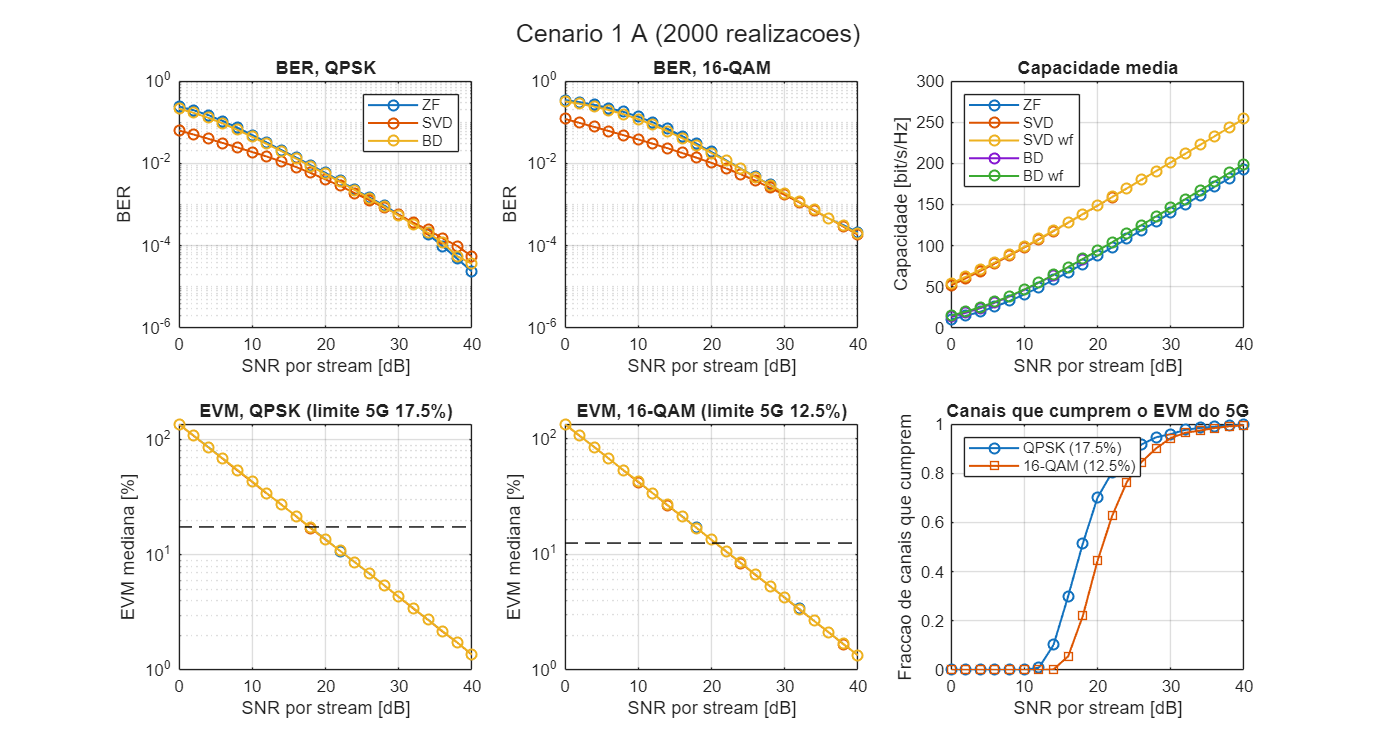
\includegraphics[width=0.9\linewidth]{IMAGENS/F1_C1A}
  \caption{Fase 1, cenário 1 A (16 utilizadores $\times$ 1 antena): BER, capacidade, EVM e fração de canais que cumprem o limiar de EVM.}
  \label{fig:f1_1A}
\end{figure}

Com 16 utilizadores de uma antena, a BD reduz-se a anular a interferência entre \emph{streams} como o ZF; a diferença é a potência: o ZF iguala a SNR de todos os \emph{streams}, gastando potência nos canais piores, e a BD reparte-a por igual. Daí a pequena vantagem da BD na capacidade (93,9 contra 87,7\,bit/s/Hz a 20\,dB, $+7\,\%$). O SVD (148,6\,bit/s/Hz) é um limite superior: exige receptores cooperantes, impossível com uma antena por utilizador. O EVM é igual nas três técnicas (as curvas sobrepõem-se), como previsto na Secção~\ref{sec:sinais}. A BER decresce devagar com a SNR (o ZF com $N_t=N_s$ tem diversidade de ordem 1). O SVD tem a BER mais baixa a SNR baixa, mas as três técnicas aproximam-se acima de 25\,dB e o ZF acaba ligeiramente abaixo. No SVD a SNR dos \emph{streams}, $\gamma\sigma_i^2$, é desigual e os mais fracos dominam a BER média, ao passo que o ZF iguala-a.

\subsubsection{Cenário 1 B}
\begin{figure}[H]
  \centering
  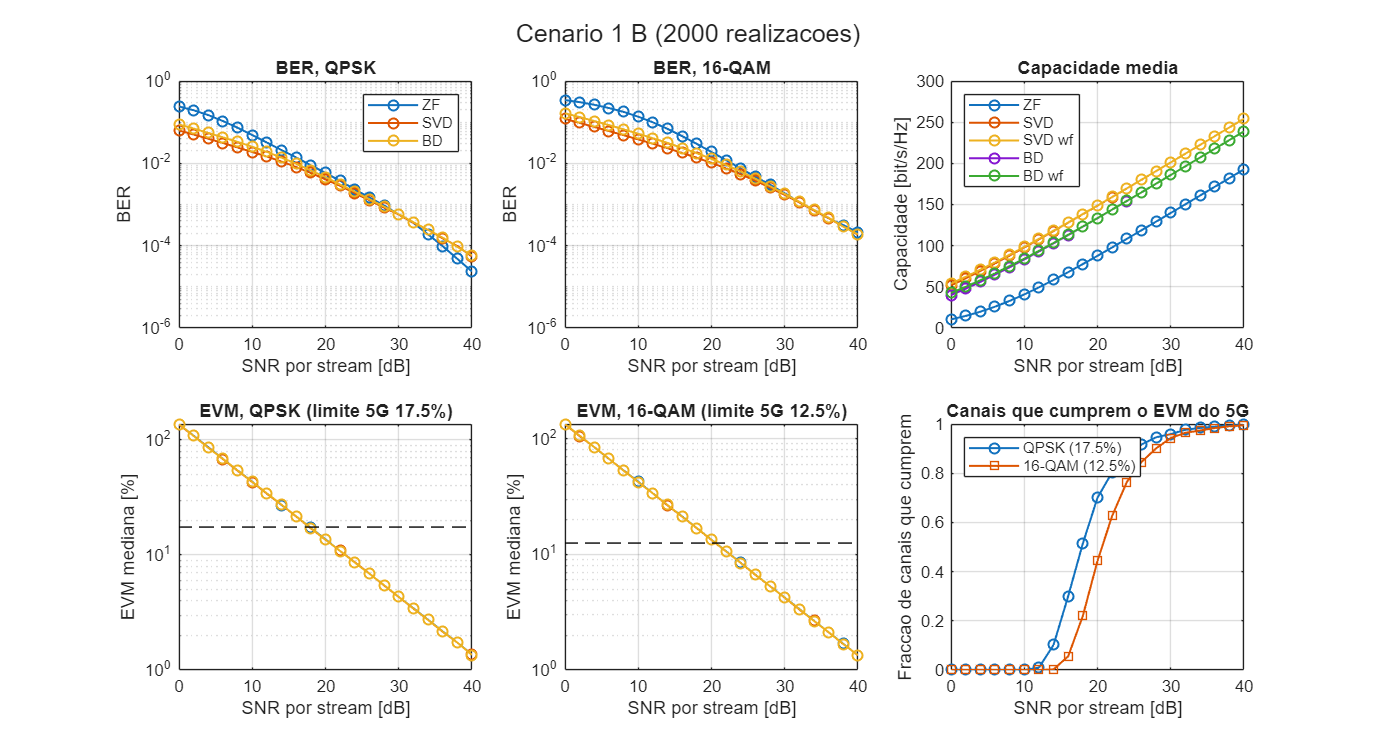
\includegraphics[width=0.9\linewidth]{IMAGENS/F1_C1B}
  \caption{Fase 1, cenário 1 B (2 utilizadores $\times$ 8 antenas): BER, capacidade, EVM e fração de canais que cumprem o limiar de EVM.}
  \label{fig:f1_1B}
\end{figure}

Com 2 utilizadores de 8 antenas, a BD só anula a interferência entre utilizadores; os 8 \emph{streams} de cada um são separados pelo seu receptor $\mathbf{G}_j$. Aproveita assim a diversidade dos receptores, o que o ZF (que trata os 16 \emph{streams} como utilizadores independentes) não faz: 133,4\,bit/s/Hz contra 87,7, $+52\,\%$, e 90\,\% do limite do SVD. O ZF e o SVD não dependem do agrupamento das antenas, pelo que têm o mesmo desempenho que em 1 A. A BER da BD acompanha a do SVD, abaixo da do ZF a SNR baixa.

\subsubsection{Cenário 2 A}
\begin{figure}[H]
  \centering
  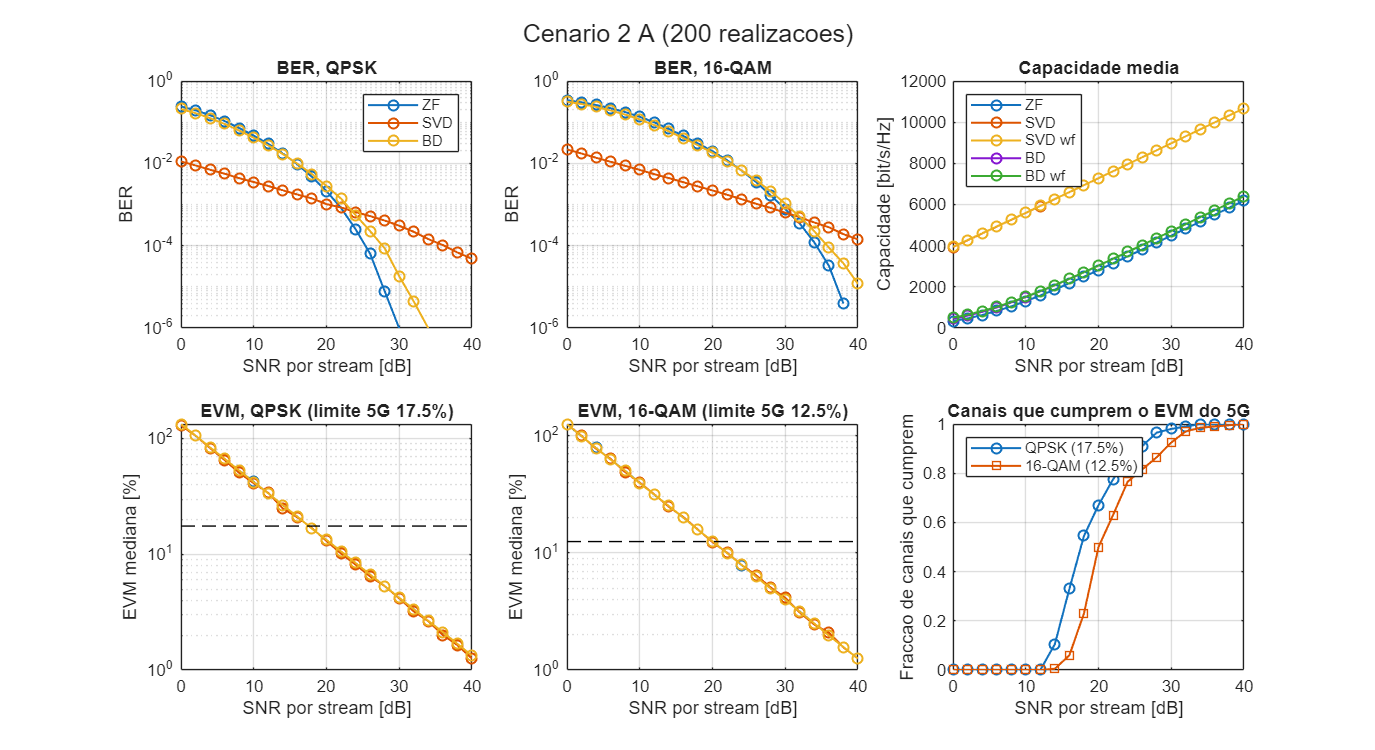
\includegraphics[width=0.9\linewidth]{IMAGENS/F1_C2A}
  \caption{Fase 1, cenário 2 A (512 utilizadores $\times$ 1 antena): BER, capacidade, EVM e fração de canais que cumprem o limiar de EVM.}
  \label{fig:f1_2A}
\end{figure}

Com 512 antenas e 512 utilizadores, a capacidade multiplica por 32 no ZF (2816 contra 88\,bit/s/Hz): cresce linearmente com $N_s$. O SVD cresce mais, $\times49$ (7278 contra 149), porque o maior valor singular de $\mathbf{H}$ cresce com $\sqrt{N}$; é o único que ganha com a dimensão da matriz, mas continua a precisar de receptores cooperantes. A BD fica $+8\,\%$ acima do ZF (3032\,bit/s/Hz). Na BER o cruzamento vê-se melhor: o SVD é melhor abaixo de cerca de 20\,dB, mas decresce devagar (ainda acima de $10^{-5}$ a 40\,dB), enquanto o ZF e a BD descem depressa. A descida do ZF acima de cerca de 22\,dB deve ser lida com cautela: com $D=200$ realizações, os canais raros quase singulares, que dominam a BER média, deixam de ser amostrados.

\subsubsection{Cenário 2 B}
\begin{figure}[H]
  \centering
  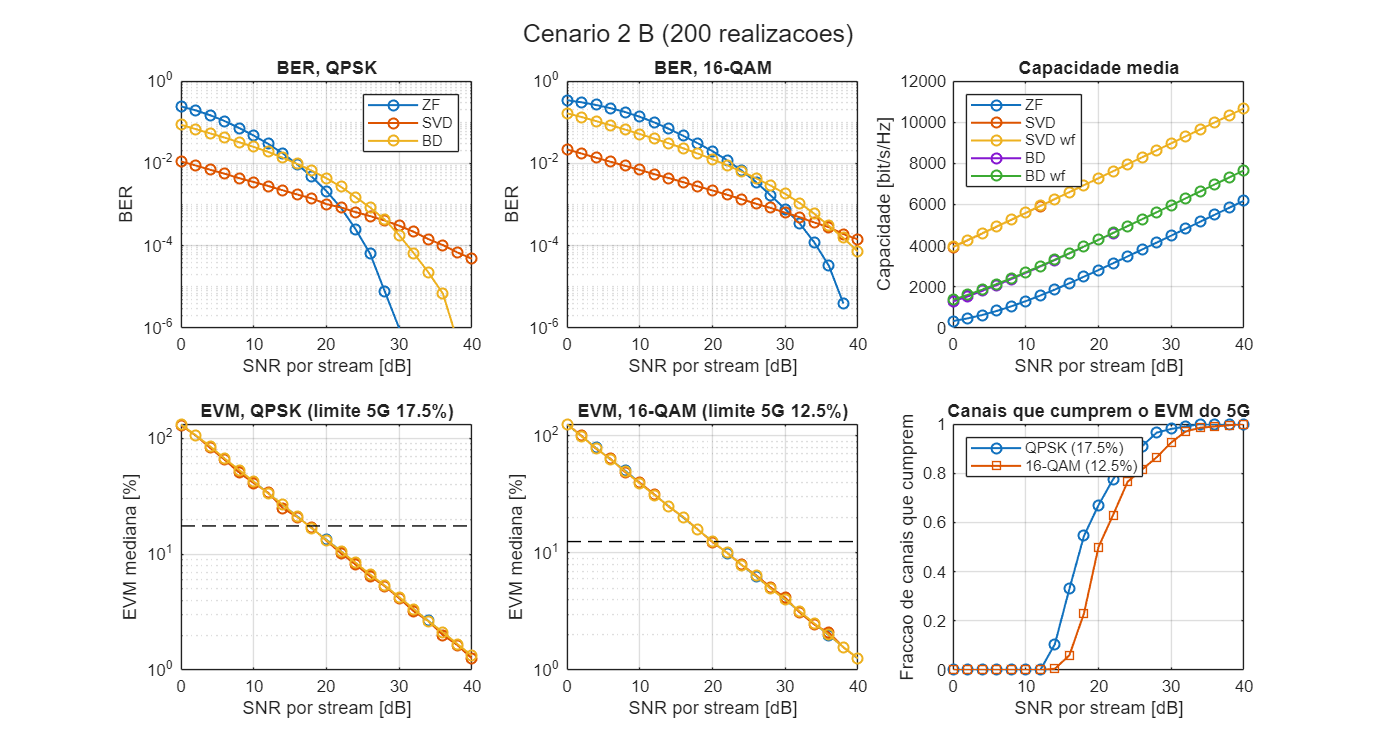
\includegraphics[width=0.9\linewidth]{IMAGENS/F1_C2B}
  \caption{Fase 1, cenário 2 B (64 utilizadores $\times$ 8 antenas): BER, capacidade, EVM e fração de canais que cumprem o limiar de EVM.}
  \label{fig:f1_2B}
\end{figure}

Com 64 utilizadores de 8 antenas, a BD atinge 4282\,bit/s/Hz, $+52\,\%$ face ao ZF. Em 1 B e em 2 B cada utilizador fica com um canal equivalente $8\times8$ (o espaço nulo dos restantes tem dimensão 8), e a capacidade da BD por utilizador é a mesma, 66,7\,bit/s/Hz: a BD escala com o número de utilizadores, mas não aproveita o ganho de $N_t$ como o SVD. Por isso, em 2 B a BD só atinge 59\,\% do limite do SVD (90\,\% em 1 B). Na BER a BD fica entre o ZF e o SVD: melhor do que o ZF abaixo de cerca de 20\,dB e pior acima.

\subsubsection{Comparação de capacidade e complexidade}
\label{sec:comp1}
\begin{table}[H]
  \centering
  \caption{Capacidade média a 20\,dB por subportadora (bit/s/Hz), Fase 1.}
  \label{tab:cap1}
  \begin{tabular}{@{}lccccc@{}}
    \toprule
    Cenário & ZF & SVD & SVD-WF & BD & BD-WF \\
    \midrule
    1 A & 87,7 & 148,6 & 148,8 & 93,9 & 94,0 \\
    1 B & 87,7 & 148,6 & 148,8 & 133,4 & 133,6 \\
    2 A & 2816 & 7278 & 7280 & 3032 & 3033 \\
    2 B & 2816 & 7278 & 7280 & 4282 & 4287 \\
    \bottomrule
  \end{tabular}
\end{table}

A Tabela~\ref{tab:cap1} resume as capacidades a 20\,dB. Em todos os cenários a ordem é SVD $>$ BD $>$ ZF, e a BD só se afasta muito do ZF quando os utilizadores têm várias antenas. O \emph{water-filling} acrescenta pouco: cerca de 1\,\% a 10\,dB e 0,1\,\% a 20\,dB, porque quase todos os \emph{streams} já têm SNR suficiente.

\begin{table}[H]
  \centering
  \caption{Tempo de cálculo de $\mathbf{P}$ e $\mathbf{G}$ por subportadora (ms) e ordem de complexidade teórica.}
  \label{tab:compl}
  \begin{tabular}{@{}lccccl@{}}
    \toprule
    Técnica & 1 A & 1 B & 2 A & 2 B & Ordem \\
    \midrule
    ZF & 0,021 & 0,019 & 12,7 & 14,2 & $O(N^3)$ \\
    SVD & 0,031 & 0,030 & 74,2 & 71,8 & $O(N^3)$ \\
    BD ``rápida'' & 0,100 & 0,042 & 26,2 & 18,7 & $O(N^3)$ \\
    BD clássica & 2,57 & 1,20 & 34747 & 4124 & $O(K\,N^3)$ \\
    \bottomrule
  \end{tabular}
\end{table}

A Tabela~\ref{tab:compl} mostra o tempo médio de cálculo de $\mathbf{P}$ e $\mathbf{G}$ por subportadora. O ZF é a técnica mais barata. O SVD custa cerca de 1,5 a 6 vezes mais (mais com $N$ elevado). A BD clássica obriga a uma SVD por utilizador, ou seja, $K$ vezes o custo do SVD, o que a torna impraticável em Massive MIMO: 35\,s por subportadora em 2 A. Com a BD ``rápida'', que usa a inversa de $\hat{\mathbf{H}}$ por ser quadrada, o custo desce para 1,3 a 5 vezes o do ZF, mas só é possível porque $\mathbf{H}$ é quadrada. De 16 para 512 antenas o tempo do ZF cresce 600 vezes, menos do que os $32^3\approx3\times10^4$ da ordem teórica $O(N^3)$, porque com matrizes pequenas o tempo é dominado por custos fixos do Matlab. Estes tempos repetem-se em cada subportadora: para 512 subportadoras, um símbolo OFDM em 2 A custa 6,5\,s no ZF, 38\,s no SVD, 13\,s na BD rápida e 17790\,s (cerca de 5 horas) na BD clássica, quando um símbolo dura dezenas de microssegundos. A complexidade da pré-codificação totalmente digital é o principal obstáculo do Massive MIMO.

% ---------------------------------------------------------------------------
% 2.4 Fase 2
% ---------------------------------------------------------------------------
\subsection{Fase 2: Estimativa imperfeita do canal}
\label{sec:fase2}

Compararam-se ZF, SVD, BD e MMSE com três níveis de erro $\sigma_e^2$ por cenário. Cada figura mostra a BER, a capacidade, o EVM e a interferência (IUI a cheio, ISI a tracejado) para o nível intermédio; os outros níveis estão na Secção~\ref{sec:comp2}. Com o mesmo $\sigma_e^2$ a interferência é proporcional a $N_s$: para $N_s=16$ é de cerca de $1{,}8\,N_s\sigma_e^2$ (estimativa empírica), e para $N_s=512$ é 15\,dB maior. Por isso os níveis para 512 antenas são 15\,dB inferiores.

\begin{table}[H]
  \centering
  \caption{ZF, SVD e BD: interferência total prevista $1{,}8\,N_s\sigma_e^2$ e EVM de piso $100\sqrt{1{,}8\,N_s\sigma_e^2}$.}
  \label{tab:piso}
  \begin{tabular}{@{}lccc@{}}
    \toprule
    & Nível 1 & Nível 2 & Nível 3 \\
    \midrule
    $\sigma_e^2$, 16 antenas (dB) & $-40$ & $-35$ & $-30$ \\
    $\sigma_e^2$, 512 antenas (dB) & $-55$ & $-50$ & $-45$ \\
    Interferência total (dB) & $-25{,}4$ & $-20{,}4$ & $-15{,}4$ \\
    EVM de piso (\%) & 5,4 & 9,5 & 17,0 \\
    Limiar QPSK (17,5\,\%) & cumpre & cumpre & no limite \\
    Limiar 16-QAM (12,5\,\%) & cumpre & cumpre & não cumpre \\
    \bottomrule
  \end{tabular}
\end{table}

Os dois casos têm assim a mesma interferência prevista (Tabela~\ref{tab:piso}). Como $N_t=N_s$, não há excesso de antenas que atenue o erro: este passa integralmente para a interferência. Esta análise aplica-se a ZF, SVD e BD, que anulam a interferência com base em $\hat{\mathbf{H}}$; o MMSE, por ser regularizado, comporta-se de forma diferente, sobretudo com 512 antenas.

\subsubsection{Cenário 1 A}
\begin{figure}[H]
  \centering
  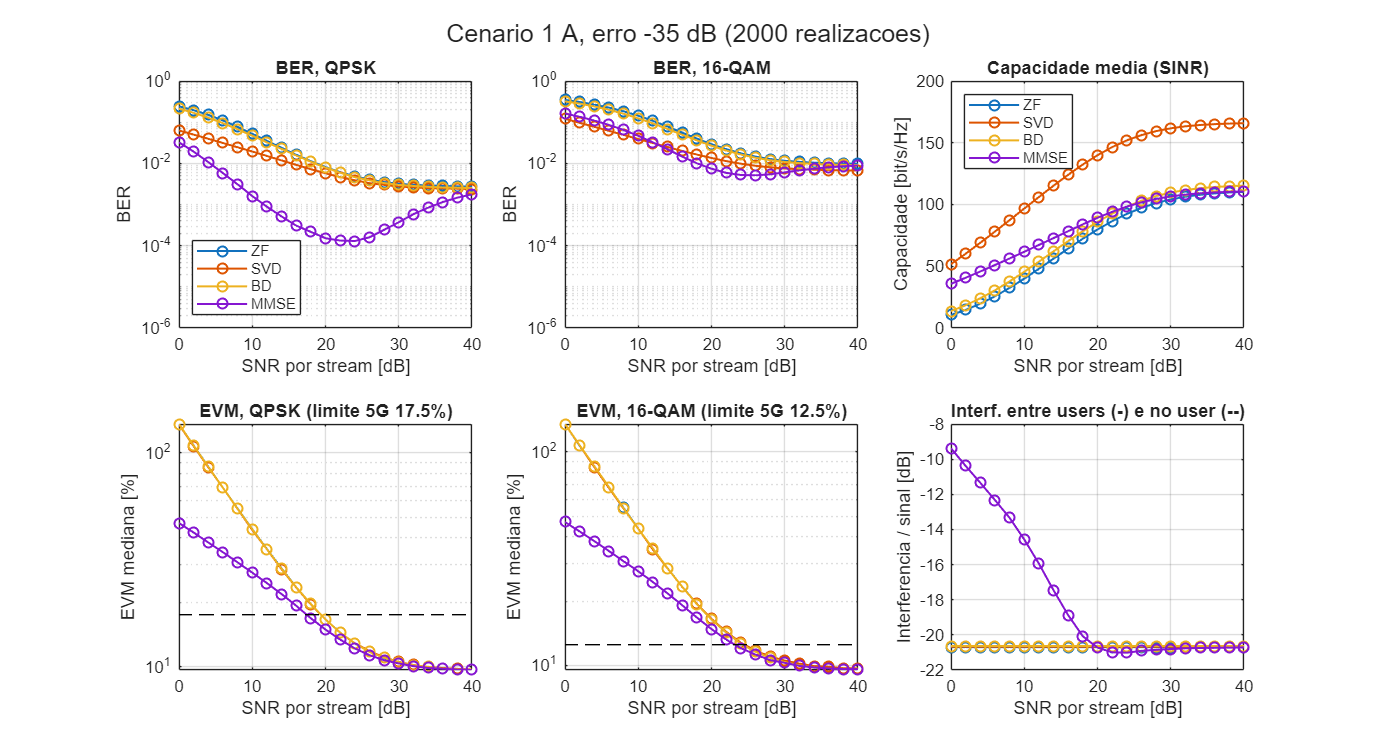
\includegraphics[width=0.9\linewidth]{IMAGENS/F2_C1A_35}
  \caption{Fase 2, cenário 1 A, $\sigma_e^2=-35$\,dB: BER, capacidade, EVM e interferência.}
  \label{fig:f2_1A}
\end{figure}

Com $\sigma_e^2=-35$\,dB, a IUI a 20\,dB é de $-20{,}7$\,dB em ZF, SVD e BD e não desce com a SNR. Estas técnicas cancelam a interferência só em relação a $\hat{\mathbf{H}}$, e o erro deixa uma fuga $A_{ij}\neq0$ igual nas três: com estimativa imperfeita a interferência passa a ser independente da técnica. A capacidade do ZF cai de 87,7 para 79,8\,bit/s/Hz (a do SVD de 148,6 para 139,9) e cresce muito mais devagar com a SNR. O EVM deixa de descer abaixo do piso de 9,5\,\%, e a SNR mínima sobe de 17,8 para 19,4\,dB em QPSK e de 20,6 para 24,4\,dB em 16-QAM. A BER de ZF, SVD e BD estabiliza em cerca de $4\times10^{-3}$ (QPSK) e $10^{-2}$ (16-QAM) acima de 30\,dB. O MMSE tem mais IUI a SNR baixa, que desce até ao patamar das outras técnicas por volta dos 20\,dB, mas compensa com menos ruído: a capacidade e a BER são melhores até cerca de 25\,dB (a 20\,dB, 89,2\,bit/s/Hz, e BER em QPSK de $10^{-4}$ por volta dos 22\,dB), e a SNR mínima é de 17,4\,dB (QPSK) e 23,2\,dB (16-QAM). A SNR alta junta-se às outras técnicas.

\subsubsection{Cenário 1 B}
\begin{figure}[H]
  \centering
  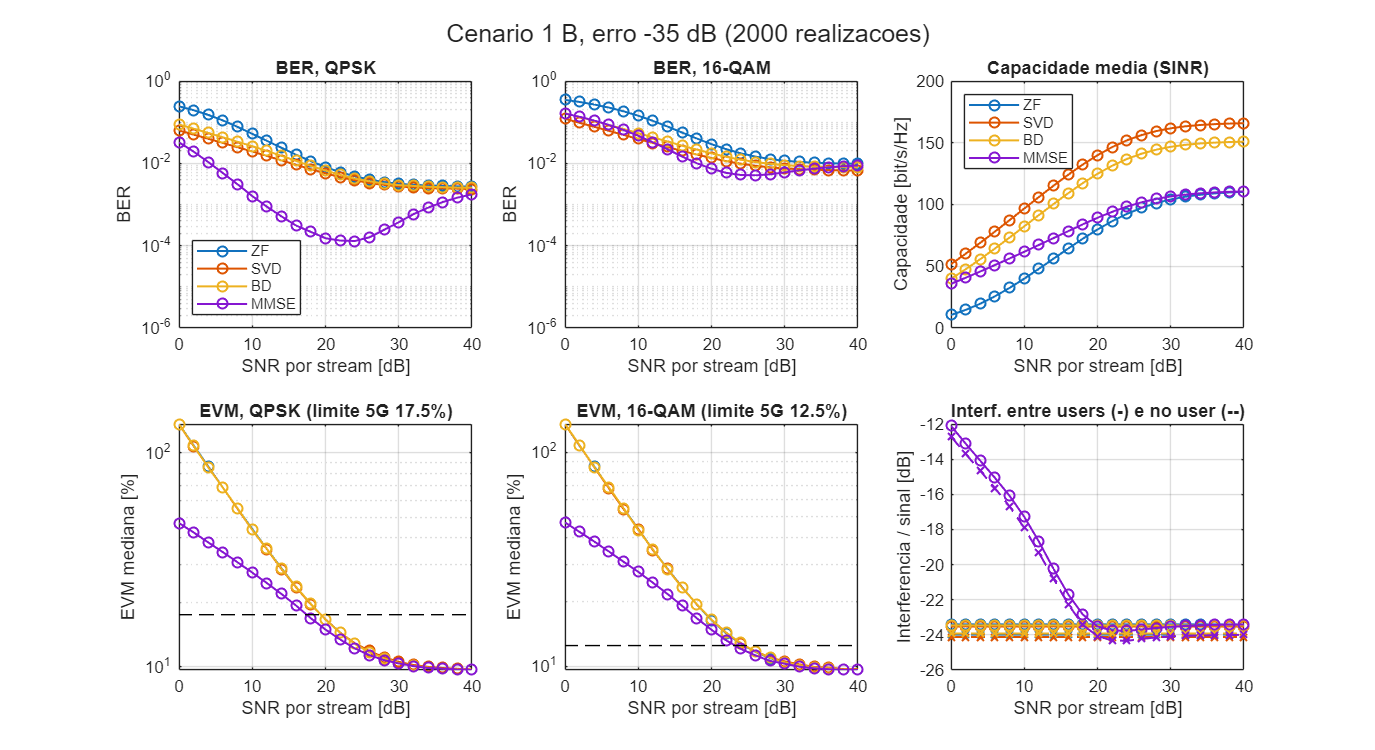
\includegraphics[width=0.9\linewidth]{IMAGENS/F2_C1B_35}
  \caption{Fase 2, cenário 1 B, $\sigma_e^2=-35$\,dB: BER, capacidade, EVM e interferência.}
  \label{fig:f2_1B}
\end{figure}

A interferência total é semelhante à de 1 A, mas divide-se entre IUI e ISI: a IUI, $-23{,}4$\,dB, é cerca de 3\,dB inferior. Na Fase 1 a ISI era nula no SVD e na BD, porque o receptor de cada utilizador separa os seus \emph{streams}; com $\hat{\mathbf{H}}$ deixa de ser, porque $\mathbf{G}_j$ também é calculado com a estimativa. A BD continua acima do ZF (124,8 contra 79,8\,bit/s/Hz) e a 89\,\% do SVD (139,9). O MMSE (89,2) fica ao nível do ZF porque, ao contrário da BD, trata cada \emph{stream} em separado e não tira partido do receptor de 8 antenas.

\subsubsection{Cenário 2 A}
\begin{figure}[H]
  \centering
  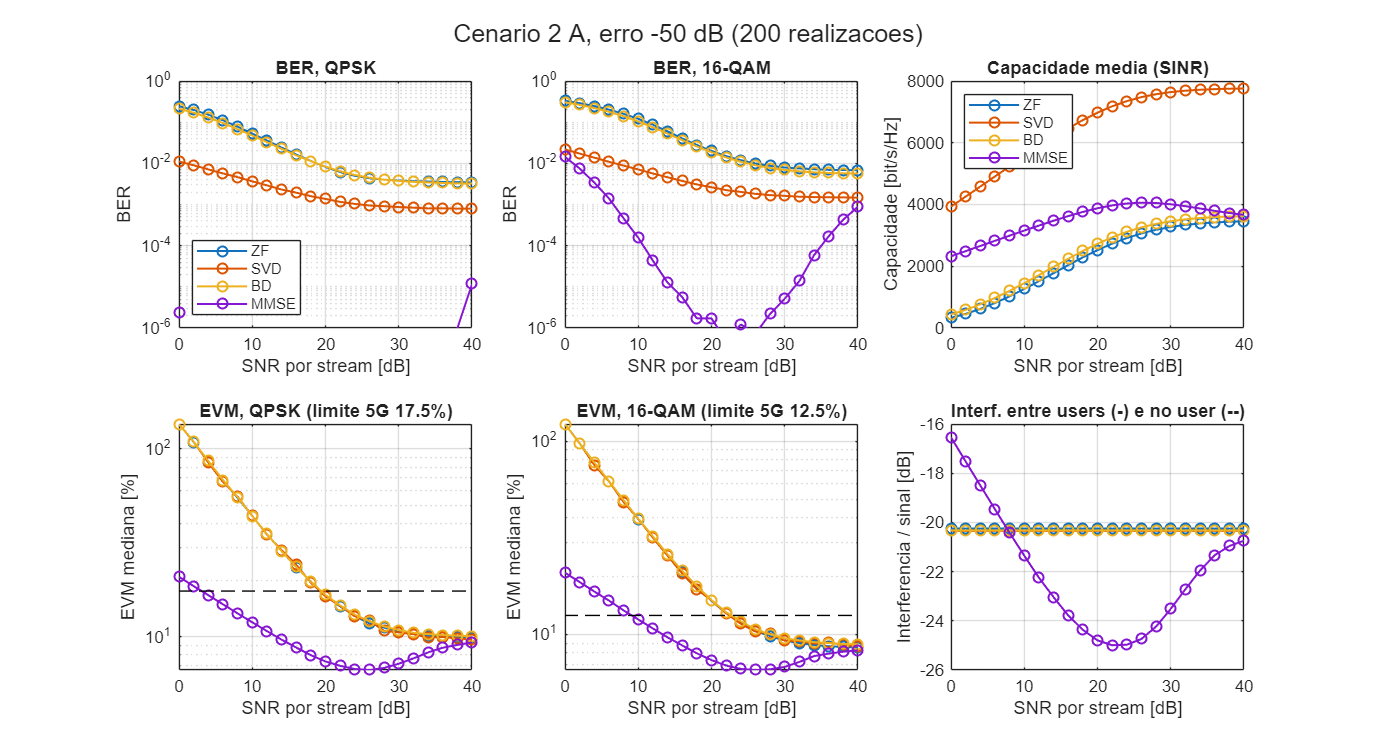
\includegraphics[width=0.9\linewidth]{IMAGENS/F2_C2A_50}
  \caption{Fase 2, cenário 2 A, $\sigma_e^2=-50$\,dB: BER, capacidade, EVM e interferência.}
  \label{fig:f2_2A}
\end{figure}

Com $\sigma_e^2=-50$\,dB, a IUI de ZF, SVD e BD é de $-20{,}3$\,dB, igual à de 1 A com $-35$\,dB: com 512 antenas o erro tolerável é 15\,dB menor. Com $-35$\,dB a interferência prevista seria de $-5$\,dB. Para cumprir o limiar do 16-QAM seria preciso $\sigma_e^2\lesssim-48$\,dB nestas três técnicas, contra $-33$\,dB com 16 antenas. O MMSE é a exceção: a regularização limita a amplificação do ruído e do erro nas direcções de canal fracas, que numa matriz quadrada $512\times512$ são muitas. A 20\,dB a IUI é de $-24{,}8$\,dB, a capacidade de 3878\,bit/s/Hz (contra 2522 no ZF e 2729 na BD) e os limiares de EVM cumprem-se com 3,1\,dB (QPSK) e 9,1\,dB (16-QAM) de SNR, contra 19 a 22\,dB. Estes valores são os previstos pela teoria: com $N=512$ o EVM do MMSE é aproximadamente $100/(\gamma N)^{1/4}$, que dá 17,5\,\% e 12,5\,\% para 3\,dB e 9\,dB. Em QPSK não se mediram erros de bit entre cerca de 2 e 38\,dB. Com $-45$\,dB só o MMSE cumpre o 16-QAM. A vantagem do MMSE está numa janela de SNR: a capacidade tem um máximo, perto de 4000\,bit/s/Hz, por volta dos 25\,dB e desce depois, e a IUI volta a subir até ao patamar de $-20$\,dB das outras técnicas a 40\,dB. A regularização $\alpha=1/\gamma$ diminui com a SNR e o MMSE tende para o ZF, deixando de proteger contra o erro de estimação. Uma regularização que também tivesse o erro em conta deveria atenuar isto (não foi simulada).

\subsubsection{Cenário 2 B}
\begin{figure}[H]
  \centering
  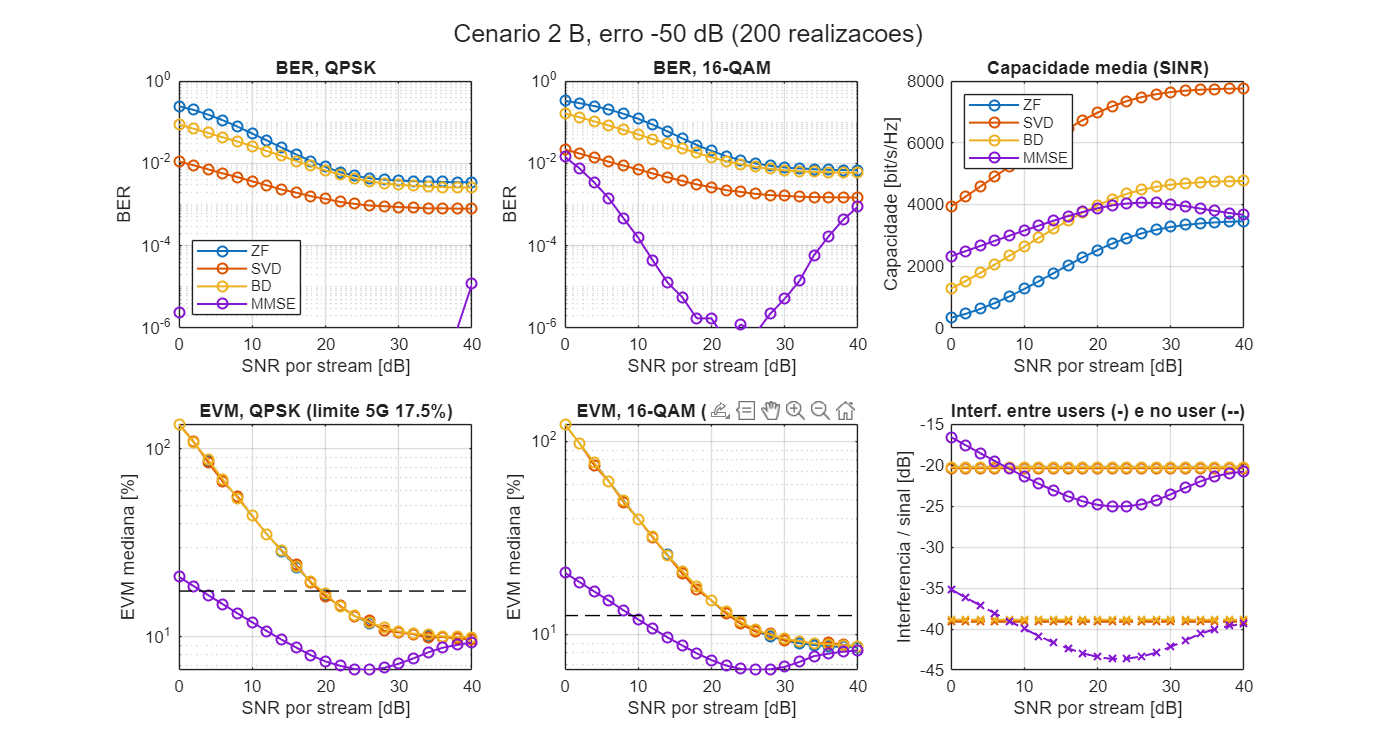
\includegraphics[width=0.9\linewidth]{IMAGENS/F2_C2B_50}
  \caption{Fase 2, cenário 2 B, $\sigma_e^2=-50$\,dB: BER, capacidade, EVM e interferência.}
  \label{fig:f2_2B}
\end{figure}

A IUI de ZF, SVD e BD é igual à de 2 A. A ISI é cerca de 18\,dB inferior à IUI (7 \emph{streams} do mesmo utilizador em 511), pelo que a interferência é quase só entre utilizadores. A BD tem vantagem sobre o ZF (3976 contra 2522\,bit/s/Hz, $+58\,\%$). A 20\,dB o MMSE (3878\,bit/s/Hz) fica perto da BD sem exigir receptores de várias antenas, com menos IUI ($-24{,}9$\,dB contra $-20{,}3$) e com SNR mínima de 3,1\,dB (QPSK) e 9,1\,dB (16-QAM). A SNR alta a BD ultrapassa-o (cerca de 4800 contra 3700\,bit/s/Hz a 40\,dB).

\subsubsection{Comparação entre cenários e níveis de erro}
\label{sec:comp2}
\begin{table}[H]
  \centering
  \caption{IUI mediana (dB) a 20\,dB, Fase 2.}
  \label{tab:iui}
  \footnotesize
  \begin{tabular}{@{}llcccc@{}}
    \toprule
    Cenário & $\sigma_e^2$ (dB) & ZF & SVD & BD & MMSE \\
    \midrule
    1 A & $-40$ & $-25{,}7$ & $-25{,}7$ & $-25{,}7$ & $-23{,}9$ \\
     & $-35$ & $-20{,}7$ & $-20{,}7$ & $-20{,}6$ & $-20{,}7$ \\
     & $-30$ & $-15{,}7$ & $-15{,}7$ & $-15{,}7$ & $-16{,}6$ \\
    1 B & $-40$ & $-28{,}4$ & $-28{,}5$ & $-28{,}5$ & $-26{,}6$ \\
     & $-35$ & $-23{,}4$ & $-23{,}5$ & $-23{,}5$ & $-23{,}5$ \\
     & $-30$ & $-18{,}4$ & $-18{,}5$ & $-18{,}4$ & $-19{,}3$ \\
    2 A & $-55$ & $-25{,}3$ & $-25{,}3$ & $-25{,}3$ & $-25{,}9$ \\
     & $-50$ & $-20{,}2$ & $-20{,}3$ & $-20{,}3$ & $-24{,}8$ \\
     & $-45$ & $-15{,}2$ & $-15{,}2$ & $-15{,}2$ & $-22{,}4$ \\
    2 B & $-55$ & $-25{,}4$ & $-25{,}3$ & $-25{,}3$ & $-26{,}0$ \\
     & $-50$ & $-20{,}3$ & $-20{,}4$ & $-20{,}3$ & $-24{,}9$ \\
     & $-45$ & $-15{,}2$ & $-15{,}2$ & $-15{,}2$ & $-22{,}4$ \\
    \bottomrule
  \end{tabular}
\end{table}

A Tabela~\ref{tab:iui} mostra a IUI mediana a 20\,dB. Em ZF, SVD e BD é igual entre técnicas e segue a previsão da Tabela~\ref{tab:piso}: $-25{,}7$, $-20{,}7$ e $-15{,}7$\,dB em 1 A e $-25{,}3$, $-20{,}2$ e $-15{,}2$\,dB em 2 A, ou seja, valores iguais com 512 antenas e níveis de erro 15\,dB menores. Em 1 B a IUI é cerca de 3\,dB inferior à de 1 A, porque a interferência passa a dividir-se com a ISI; em 2 B é igual à de 2 A. O MMSE tem menos IUI com 512 antenas ($-22{,}4$ a $-26{,}0$\,dB) e valores próximos dos das outras técnicas com 16 antenas.

\begin{table}[H]
  \centering
  \caption{SNR mínima (dB) para cumprir o limiar de EVM, Fase 2 (--: não cumpre).}
  \label{tab:snrmin}
  \footnotesize
  \begin{tabular}{@{}llcccccccc@{}}
    \toprule
    & & \multicolumn{4}{c}{QPSK} & \multicolumn{4}{c}{16-QAM} \\
    \cmidrule(lr){3-6}\cmidrule(l){7-10}
    Cen. & $\sigma_e^2$ & ZF & SVD & BD & MMSE & ZF & SVD & BD & MMSE \\
    \midrule
    1 A & $-40$ & 18,3 & 18,2 & 18,3 & 16,6 & 21,5 & 21,5 & 21,5 & 20,7 \\
     & $-35$ & 19,4 & 19,4 & 19,4 & 17,4 & 24,4 & 24,5 & 24,2 & 23,2 \\
     & $-30$ & 29,3 & 29,9 & 29,2 & 26,0 & -- & -- & -- & -- \\
    1 B & $-40$ & 18,3 & 18,2 & 18,3 & 16,6 & 21,5 & 21,5 & 21,6 & 20,7 \\
     & $-35$ & 19,4 & 19,4 & 19,4 & 17,4 & 24,4 & 24,5 & 24,6 & 23,2 \\
     & $-30$ & 29,3 & 29,9 & 30,3 & 26,0 & -- & -- & -- & -- \\
    2 A & $-55$ & 18,4 & 18,1 & 18,3 & 3,1 & 20,5 & 20,5 & 20,5 & 9,0 \\
     & $-50$ & 19,4 & 19,2 & 19,4 & 3,1 & 22,5 & 22,4 & 22,7 & 9,1 \\
     & $-45$ & 36,8 & -- & -- & 3,2 & -- & -- & -- & 9,6 \\
    2 B & $-55$ & 18,4 & 18,1 & 18,2 & 3,1 & 20,5 & 20,5 & 20,4 & 9,0 \\
     & $-50$ & 19,4 & 19,2 & 19,5 & 3,1 & 22,5 & 22,4 & 22,8 & 9,1 \\
     & $-45$ & 36,8 & -- & 31,9 & 3,2 & -- & -- & -- & 9,6 \\
    \bottomrule
  \end{tabular}
\end{table}

A Tabela~\ref{tab:snrmin} mostra a SNR mínima para cumprir os limiares de EVM. No nível 1 a SNR mínima sobe pouco face à Fase 1 (0,4 a 1\,dB). No nível 2 sobe 2,5 a 4\,dB em 16-QAM. No nível 3 o 16-QAM nunca cumpre o limiar, por o piso (17\,\%) o exceder, e o QPSK só com 29 a 30\,dB (16 antenas); com 512 antenas só o ZF (e a BD em 2 B) o cumpre, a 32 a 37\,dB. O MMSE é a técnica que melhor resiste: com 16 antenas reduz a SNR mínima em cerca de 1 a 3\,dB, e com 512 antenas é a única que cumpre os limiares em todos os níveis testados, mas só numa janela de SNR (cenário 2 A).

\clearpage
